\subsection{Dreamfusion}\label{dreamfusion}

DreamFusion, a concept introduced by \citeauthor{pooleDreamfusion}, represents a significant advancement in the field of 3D modeling. Building upon Neuronal Radiance Fields, DreamFusion employs a novel technique called Score Distillation Sampling (SDS) to create coherent 3D objects and scenes from diverse text prompts. Unlike traditional methods that rely on pre-existing images of an object from various angles, DreamFusion generates these images during training using a diffusion model.

A key aspect of DreamFusion is its use of Differentiable Image Parameterization (DIP) \citep{mordvintsevDIP}, a method that allows for the parametrization of images through parameters (\( \theta \)) and a differentiable generator (\( g \)). This generator transforms parameters \( \theta \) into an image \( \mathbf{x} = g(\theta) \), offering refined optimization even at the pixel level \citep{pooleDreamfusion}. This technique marks a shift from the conventional approach of diffusion models, which usually produce outputs similar to their training data. In DreamFusion, the parameters \( \theta \) define 3D volumes, with \

The mathematical foundation of Score Distillation Sampling in DreamFusion starts with minimizing a diffusion training loss with respect to a generated data point \( \mathbf{x} = g(\theta) \), formulated as \[ \theta^{*} = \text{arg min}_{\theta} \mathcal{L}_{\text{Diff}}(\phi, \mathbf{x} = g(\theta)) \]. This equation seeks the optimal set of parameters (\( \theta \)) that produce the most accurate 3D model in correspondence with the text input \citep{pooleDreamfusion}.
  
The computation of the gradient of the loss function \( \mathcal{L}_{\text{Diff}} \) is crucial in determining the direction for adjusting the parameters \( \theta \) to reduce the loss. However, this computation, represented as \( \nabla_{\theta}\mathcal{L}_{\text{Diff}}(\phi,\mathbf{x}=g(\theta)) \), is typically resource-intensive and complex, involving expensive Jacobian terms. To address this, DreamFusion employs a method that simplifies the optimization process by omitting certain Jacobian terms, yet still provides a reliable direction for adjusting \( \theta \) to minimize the loss.

The SDS approach in DreamFusion is an intuitive and robust method for text-to-3D synthesis. It is based on perturbing an image \( x \) with random noise at a specific timestep \( t \), and then computing an update direction using the score function of the diffusion model to move towards regions of higher density. This methodology is anchored in a weighted probability density distillation loss, which incorporates learned score functions from the diffusion model.

The primary SDS function used in DreamFusion can be summarized as:

\[
\nabla_{\theta}\mathcal{L}_{\text{SDS}}(\phi,\mathbf{x}=g(\theta))\triangleq\mathbb{E}_{t,\epsilon}\left[w(t)\left(\hat{\epsilon}_{\phi}({\mathbf{z}}_{t};y,t)-\epsilon\right){\partial\mathbf{x}\frac\partial\theta}\right]
\]

Here, \( w(t) \) is a weighting term, \( \hat{\epsilon}_{\phi}({\mathbf{z}}_{t};y,t) \) is the predicted noise, and \( \epsilon \) is the actual noise. The gradient of the image with respect to the parameters is denoted by \( {\partial\mathbf{x}\frac\partial\theta} \). This formula efficiently guides the optimization of the parameters \( \theta \), aligning the generated data with the predictions of the diffusion model.

Furthermore, the KL Divergence, as represented in the equation 

\[
\nabla_{\theta}\mathcal{L}_{\text{SDS}}(\phi, \mathbf{x} = g(\theta)) = \nabla_{\theta}\mathbb{E}_t \left[ \frac{\sigma_t}{\alpha_t} w(t) \text{KL}(q(\mathbf{z}_t | g(\theta); y, t) || p_{\phi}(\mathbf{z}_t; y, t)) \right]
\]

quantifies the divergence between two probability distributions, further refining the process of parameter optimization in DreamFusion. This KL Divergence term helps in fine-tuning the model's alignment with the textual input and enhances the fidelity of the generated 3D models.

\begin{figure}[ht]
  \centering
    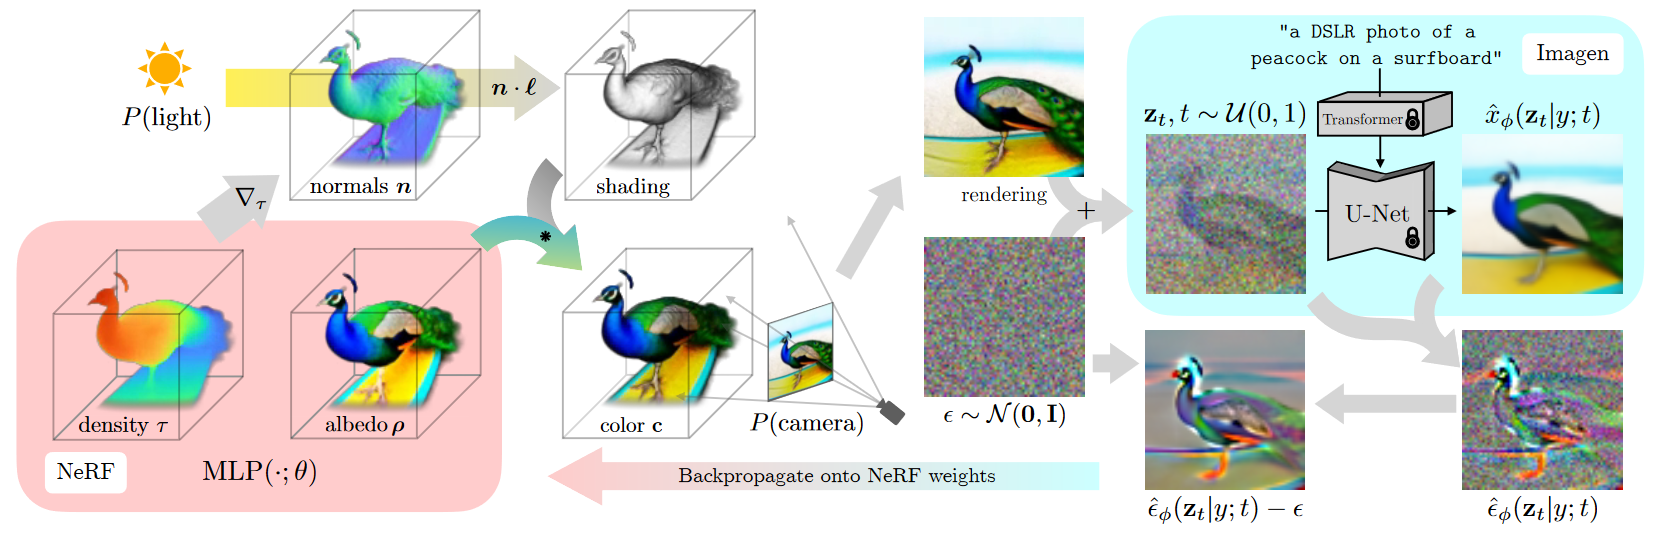
\includegraphics[width=1\columnwidth]{figures/Dreamfusion.png}
    \caption{Summatized functionality of Dreamfusion}\label{fig:figureDreamfusion}
  \end{figure}

